\section{Extensibility of \texttt{ProcessTensors.jl} and its roadmap}
\label{sec:roadmap}

So far, we have demonstrated a broad range of workflows already available in \texttt{ProcessTensors.jl}, from the construction and compression of process tensors to their interrogation with instruments and testers.
Nevertheless, the present implementation should be viewed as a foundation rather than a complete endpoint.
A central motivation for developing \texttt{ProcessTensors.jl} as an open-source package is to provide an interface that can continue to grow with new process tensor algorithms, new classes of environments, and new operational tools, while retaining a common ITensor-based language.
We have therefore designed the present API with room for extensions that may be contributed and refined by the wider community.
Below we outline several directions that we consider particularly natural continuations of the current architecture, both for broadening the physical problems that can be represented and for improving the numerical construction of PT--MPOs.

%%%%%%%%%%%%%%%%%%%%%%%%%%%%%%%%%%%%%%%%%%%%%%%%%%%%%%%%%%%%%%%%%%%%%%%%%%%
\subsection{Extending baths and measurement interfaces}
\label{subsec:roadmap-baths-instruments}

One of the most important missing environment classes in the current implementation is a fermionic bath. 
Fermionic reservoirs arise naturally in quantum-transport scenarios, where a small localized electronic system is coupled to extended electronic leads~\cite{meir1992landauer,wojtowicz2021extended,nusseler2020fermionic,bulla2008nrg,cirio2023pseudofermion,landi2022boundary}.
A paradigmatic example is the resonant-level model, which has already been treated directly within ACE using the localized fermionic level as the system and the discretized lead modes as independent environmental degrees of freedom~\cite{Cygorek2022}.
The ITensor ecosystem already provides \texttt{Fermion} and \texttt{Electron} site types together with fermionic creation and annihilation operators, fermion-parity quantum numbers, and Jordan--Wigner string operators required to represent anticommutation relations in tensor-network calculations.
A natural extension of \texttt{ProcessTensors.jl} would therefore be to introduce corresponding fermionic Hilbert-space sites and to carry their parity structure consistently through the existing Hilbert-to-Liouville mapping.
In Liouville space, left and right multiplication by fermionic operators must preserve the appropriate parity signs on the ket and bra sectors; once these superoperators are defined, they can enter the same Liouvillian and propagator routines presently used by bosonic and spin degrees of freedom.
A \texttt{FermionicMode} and corresponding fermionic bath container could then expose this construction through the same bath-mode interface used elsewhere in the package, allowing the resulting microscopic propagators to be compressed into PT--MPOs without requiring a separate process tensor representation.

The instrumentation layer can likewise be made more operational.
The current instrument primitives are sufficient to compose state preparations, observable measurements, projections, and more general maps, and therefore already allow many POVM-based protocols to be represented.
However, POVMs are not yet exposed as a first-class user abstraction that groups a complete set of measurement outcomes into a single operational object.
A dedicated POVM utility could provide a collection of positive effects \(\{E_a\}\), verify the completeness condition \(\sum_a E_a=\mathbb{I}\) when appropriate, associate each outcome with its corresponding single-leg readout, and, when a post-measurement state update is required, connect the effects to a compatible quantum instrument.
Such an interface would make experimentally motivated measurement protocols considerably easier to express than assembling each outcome manually from lower-level preparation and measurement primitives, while remaining naturally compatible with the existing \texttt{AbstractInstrument} hierarchy and \texttt{InstrumentSeq} schedules.

A further extension concerns dissipative bath modes.
At present, the ACE path constructs each microscopic mode influence through a closed Hilbert-space unitary channel, even though the underlying builder infrastructure already contains a Liouville-space propagator path.
This makes mode-local Markovian dissipation a particularly direct addition.
Bath modes could be supplied with jump operators and rates, in the same spirit as the dissipative system objects already used elsewhere in the package.
A prospective user interface could add the existing \texttt{jump\_ops} convention directly to a bath-mode constructor:
%
\begin{juliacode}[
    caption={Prospective interface to define a lossy bosonic bath mode.},
    label={lst:roadmap-dissipative-bath-mode},
]
loss = OpSum()
loss += kappa, "A", 1

mode = bosonic_mode(
    bath_sites_L,
    H_E,
    rho_E0_L;
    coupling=H_SE,
    jump_ops=[loss],
)
\end{juliacode}
%
The bath-mode propagator would then determine whether a mode is closed and unitary or whether its timestep map must instead be generated from a Liouvillian containing the Hamiltonian, system--mode coupling, and mode-local jump operators.
Importantly, this changes the microscopic mode propagator rather than the ACE compression itself: once the resulting single-mode influence is represented as a PT--MPO, the existing joining and compression routines can operate on it unchanged.
This separation provides a straightforward route to damped cavity modes, lossy auxiliary modes, or locally thermalised environmental degrees of freedom without introducing a second compression formalism.

%%%%%%%%%%%%%%%%%%%%%%%%%%%%%%%%%%%%%%%%%%%%%%%%%%%%%%%%%%%%%%%%%%%%%%%%%%%
\subsection{Scalable ACE contraction and custom bath modes}
\label{subsec:roadmap-ace}

The present ACE backend combines independent mode influences sequentially, following the construction used in the original ACE toolkit~\cite{CygorekGauger2024}.
A particularly promising extension is the treelike contraction scheme introduced for ACE in Ref.~\cite{Cygorek2024Treelike}, where partial PT--MPOs are combined hierarchically rather than adding every new mode to one continuously growing process tensor.
The published construction shows that this reordering can substantially reduce the cost of the intermediate contractions, while preselection and additional compression sweeps can control the large temporary bond spaces that appear when two already-compressed PT--MPOs are joined.
From the perspective of the present API, this is naturally a new contraction strategy rather than a new process tensor type:
%
\begin{juliacode}[
    caption={Prospective tree-like ACE construction through the existing builder interface.},
    label={lst:roadmap-tree-ace},
]
pt_tree = build_process_tensor(
    system;
    method=ACE(
        cutoff=1e-10,
        compression=:canonzip,
        contraction=:tree,
        parallel=true,
        # Other ACE kwargs
    ),
    environment=environment,
    dt=dt,
    nsteps=nsteps,
)
\end{juliacode}
%
The option \texttt{contraction=:sequential} would retain the current behaviour.
Additional keyword arguments could expose treelike-specific choices such as preselection and the number of compression sweeps, without prescribing a particular internal implementation to future contributors.
This keeps the public interface compact while allowing the ACE backend to incorporate improvements developed in the broader literature.

Treelike contraction also creates a natural opportunity for parallel execution.
Independent pairs of partial PT--MPOs within the same tree level can be constructed and compressed concurrently before the next level is assembled.
A future implementation could therefore parallelise independent branches of the contraction tree while retaining the same user-facing builder.
The precise scheduling strategy should remain an implementation choice---in particular, it must balance task-level parallelism against threaded linear-algebra kernels and the memory cost of holding several intermediate PT--MPOs simultaneously---but the treelike organization provides the required independence without any change to the mathematical object returned to the user.

ACE can also be extended from static to explicitly time-dependent bath modes.
The current single-mode construction reuses a timestep propagator when the bath Hamiltonian is time independent.
Allowing the Hamiltonian of a bath mode, or its coupling to the system, to depend on time would instead let the builder generate a mode propagator appropriate to each interval \([t_k,t_{k+1}]\).
At the API level, this could be expressed directly through the bath-mode Hamiltonian or coupling object, for example by permitting callable or otherwise time-dependent operator coefficients.
A driven spin mode and its process tensor could then be constructed through a prospective interface such as in Listing~\ref{lst:roadmap-driven-bath-mode}:
%
\begin{juliacode}[
    caption={Prospective ACE construction for a bath mode with a time-dependent Hamiltonian.},
    label={lst:roadmap-driven-bath-mode},
]
function H_E(t)
    H = OpSum()
    H += omega_E / 2, "Sz", 1
    H += drive * cos(nu * t), "Sx", 1
    return H
end

driven_mode = spin_mode(bath_sites_L, H_E, rho_E0_L; coupling=H_SE)
\end{juliacode}
%
\noindent
The ACE builder would then read the mode at the requested time and construct the corresponding microscopic timestep map before carrying out the usual PT--MPO combination and compression.
In this way driven auxiliary modes, modulated couplings, and other non-stationary environments could be introduced without changing the representation of the final process tensor.

More generally, the ACE backend provides a natural route toward user-defined baths and bath modes.
The essential requirement of ACE is not that every environmental degree of freedom belongs to one of a small number of predefined physical classes, but that the influence of each independent microscopic component can be supplied as a compatible system--mode timestep map.
Consequently, a lightweight interface for custom subtypes of \texttt{AbstractBathMode} could allow advanced users to define their own local Hilbert space, initial state, generator, and system--mode coupling while reusing the same ACE machinery for PT--MPO assembly.
The existing \texttt{BosonicMode} and \texttt{SpinMode} types would then remain convenient high-level constructors, while fermionic, multilevel, anharmonic, driven, or application-specific modes could enter through the same backend.
Such an extension would preserve the pedagogical simplicity of the standard API while making \texttt{ProcessTensors.jl} a substantially more general platform for constructing process tensors from microscopic models.

%%%%%%%%%%%%%%%%%%%%%%%%%%%%%%%%%%%%%%%%%%%%%%%%%%%%%%%%%%%%%%%%%%%%%%%%%%%
\subsection{Support for Gaussian baths using Feynman--Vernon approaches}
\label{subsec:roadmap-pttempo}

The ACE construction used in the present implementation is deliberately microscopic: a bath is resolved into individual modes, the influence of each mode is constructed explicitly, and the resulting process tensors are combined and compressed.
This flexibility is valuable for structured, non-Gaussian, or otherwise mode-resolved environments, but a continuum bath must first be represented by a finite collection of modes, introducing an additional bath-discretisation parameter whose convergence must be checked~\cite{cygorek2022ace}.
Fortunately, for stationary Gaussian environments there is a complementary route.
If the bath consists of non-interacting modes and is initially in a stationary thermal Gaussian state, its influence can be integrated out analytically at the level of the Feynman--Vernon influence functional~\cite{feynman1963influence,makri1995tensor}.
The bath may then be specified directly by a spectral density $J(\omega)$ and temperature rather than by an explicit list of microscopic modes.
This removes the additional error associated with discretising a continuum spectrum into finitely many bath particles, while retaining the non-Markovian temporal correlations of the bath.
The remaining numerical approximations are instead controlled by the time step, numerical quadrature, any imposed memory cutoff, and tensor-network truncation.
For Gaussian baths whose temporal correlations remain compressible, this can provide a particularly compact and accurate representation of the environment.

For a linearly coupled Gaussian bath,
%
\begin{equation}
    H_{SB} = S\otimes B,
\end{equation}
%
the spectral density and temperature determine the stationary two-time correlation function \(C(\tau)=\langle B(\tau)B(0)\rangle\).
Let \(s_k^+\) and \(s_k^-\) denote the eigenvalues of \(S\) on the forward and backward histories during the cell \([t_k,t_{k+1}]\).
The cell-integrated bath correlations, pairwise influence tensors, and full discretised Feynman--Vernon influence functional are then
%
\begin{align}
    \eta_{k-j}
    &=
    \int_{t_k}^{t_{k+1}}\!\mathrm{d}t
    \int_{t_j}^{\min(t,t_{j+1})}\!\mathrm{d}t'\,
    C(t-t'),
    \qquad j\leq k,
    \nonumber\\
    \mathcal I_{k-j}(s_k^\pm,s_j^\pm)
    &=
    \exp\!\left[
        -(s_k^+-s_k^-)
        \left(
            \eta_{k-j}s_j^+
            -\eta_{k-j}^*s_j^-
        \right)
    \right],
    \nonumber\\
    \mathcal F[\{s^\pm\}]
    &=
    \prod_{k=0}^{N-1}\prod_{j=0}^{k}
    \mathcal I_{k-j}(s_k^\pm,s_j^\pm).
    \label{eq:roadmap-feynman-vernon-influence}
\end{align}
%
Thus each influence tensor is obtained by integrating the bath correlation function over a pair of time cells, with time ordering on the diagonal cell \(j=k\). \textcolor{red}{Is this formula too heavy for the readers? Can skip it? }
TEMPO rewrites this non-local temporal object as a tensor network and repeatedly applies singular-value decompositions to retain only the relevant temporal correlations~\cite{strathearn2018tempo}.
PT-TEMPO takes the same construction one step further: rather than contracting the network for one chosen reduced-state trajectory, the system input and output legs are retained, so that the compressed influence functional becomes a reusable finite process tensor MPO~\cite{jorgensen2019pttempo}.
Once constructed, this object can be interrogated with different controls, instruments, and multitime protocols without rebuilding the bath influence, as demonstrated in existing PT-TEMPO software such as OQuPy~\cite{fux2024oqupy}.
%
\begin{figure}[t]
    \centering
    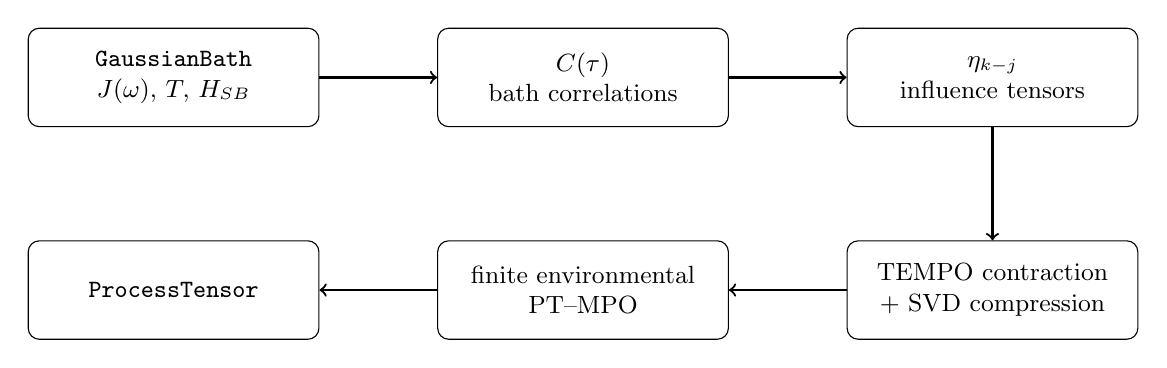
\begin{tikzpicture}[
        box/.style={
            draw,
            rounded corners,
            align=center,
            text width=3.2cm,
            minimum height=1.25cm,
            inner xsep=7pt,
            inner ysep=6pt,
            font=\small
        }
    ]
        \node[box] (bath) at (0,0)
            {$\texttt{GaussianBath}$\\$J(\omega),\,T,\,H_{SB}$};
        \node[box] (corr) at (5.2,0)
            {$C(\tau)$\\bath correlations};
        \node[box] (influence) at (10.4,0)
            {$\eta_{k-j}$\\influence tensors};
        \node[box] (tempo) at (10.4,-2.7)
            {TEMPO contraction\\+ SVD compression};
        \node[box] (pt) at (5.2,-2.7)
            {finite environmental\\PT--MPO};
        \node[box] (final) at (0,-2.7)
            {$\texttt{ProcessTensor}$};

        \draw[->, thick] (bath.east) -- (corr.west);
        \draw[->, thick] (corr.east) -- (influence.west);
        \draw[->, thick] (influence.south) -- (tempo.north);
        \draw[->, thick] (tempo.west) -- (pt.east);
        \draw[->, thick] (pt.west) -- (final.east);
    \end{tikzpicture}
    \caption{Proposed PT-TEMPO construction in the present package.
    A stationary Gaussian bath is specified directly through its spectral density, temperature, and system--bath coupling.
    The corresponding two-time correlations generate the discretised Feynman--Vernon influence tensors, which are contracted and compressed into a finite environmental PT--MPO.
    Free-system propagation is then embedded using the same convention as the existing process tensor builders, producing the standard \texttt{ProcessTensor} object used by the rest of the package.}
    \label{fig:roadmap-pttempo}
\end{figure}
%

The present source layout already provides most of the interfaces required for such a builder.
We envisage a \texttt{GaussianBath <: AbstractBath} in the existing environment module, storing three physical ingredients:
%
\begin{itemize}
    \item \textbf{Temperature $T$}: the thermal scale of the stationary Gaussian state.
    \item \textbf{Spectral density $J(\omega)$}: an Ohmic or Lorentzian form, or a user-supplied $J(\omega)$.
    \item \textbf{Linear coupling $H_{SB}$}: an operator sum validated against the Gaussian influence-functional construction.
\end{itemize}
%
Unlike the existing spin and bosonic bath containers, this object would not contain a finite collection of individual bath modes: the continuum has already been encoded in $J(\omega)$.
The coupling would then be separated internally into its system and bath components.
A PT-TEMPO method would sit beside the existing dense and ACE constructors as an \texttt{AbstractPTBuilder}, so that a prospective interface could assemble the bath and the process tensor together, as in Listing~\ref{lst:roadmap-pttempo-builder}:
%
\begin{juliacode}[
    caption={Prospective Gaussian-bath constructor and PT-TEMPO process tensor builder.},
    label={lst:roadmap-pttempo-builder},
]
bath = gaussian_bath(J, T; coupling=H_SB)

process_tensor = build_process_tensor(
    system;
    environment=bath,
    method=PTTEMPO(
        #kwargs...
    ),
    dt=dt,
    nsteps=nsteps,
)
\end{juliacode}
%
The implementation itself would reside in a new builder file beside the dense and ACE backends.
Internal helpers in this file would evaluate the bath correlations from $J(\omega)$ and $T$, construct the discretised influence tensors, and perform the TEMPO contractions and SVD compression.
A corresponding dispatch would return the same finite process tensor representation used throughout the package.
The existing ITensor infrastructure supplies the MPO representation and bond compression; the only additional numerical dependency expected at this level is an adaptive quadrature library, such as \texttt{QuadGK.jl}, for the spectral and influence-functional integrals.
Free-system propagation can then be embedded after the environmental PT--MPO has been constructed, and may be chosen trivial when only the bath influence is required.

The same Gaussian-bath abstraction could later accept fermionic hybridisation functions in place of bosonic correlation functions.
An ITensor-native route would order fermionic events along the temporal contour and encode their exchange signs through Jordan--Wigner parity strings, or equivalent parity sectors, producing an ordinary complex-valued but parity-aware influence MPO.
Fermionic influence-functional MPS calculations using closely related super-fermion and Slater-determinant machinery have already been implemented for quench dynamics of the Anderson impurity model~\cite{Park2024FermionicInfluence}.
Grassmann TEMPO provides an alternative formulation~\cite{Chen2024GTEMPO}, but incorporating its Grassmann tensor algebra would require substantial changes to the present backend.

Our immediate goal would be the standard finite-time PT-TEMPO setting: stationary thermal bosonic Gaussian baths with non-interacting modes, linear system--bath coupling, user-defined or built-in spectral densities, and controlled temporal SVD compression.
More advanced influence-functional contractions can be incorporated only after this reference implementation is established.
In particular, divide-and-conquer constructions can reduce the number of SVDs by exploiting self-similarity of Gaussian influence networks~\cite{cygorek2024sublinear}, while time-translationally invariant constructions can build matrix-product representations of the influence functional with substantially fewer tensor-network multiplications~\cite{guo2024influence}.
These algorithms provide natural future optimisation routes, but are not prerequisites for adding a self-contained PT-TEMPO backend to this package.

%%%%%%%%%%%%%%%%%%%%%%%%%%%%%%%%%%%%%%%%%%%%%%%%%%%%%%%%%%%%%%%%%%%%%%%%%%%
\subsection{Chain-mapped environments and temporal tensor-network contractions}
\label{subsec:roadmap-chainmapping}

A complementary long-term direction is to construct process tensors from an explicit tensor-network simulation of the joint system--environment dynamics.
Orthogonal-polynomial transformations map a system linearly coupled to a continuum of bosonic or fermionic modes onto a semi-infinite nearest-neighbour chain whose onsite energies, hopping amplitudes, and system--chain coupling are fixed by the bath spectral density~\cite{chin2010chain,prior2010tedopa}.
This mapping is exact before numerical truncation and places the environment in a geometry naturally suited to MPS/MPO methods.
Finite-temperature extensions such as T-TEDOPA additionally permit thermal environments to be represented through temperature-dependent chain parameters and pure-state propagation~\cite{tamascelli2019ttedopa}.
For finite simulations the chain length and, for bosons, the local Hilbert spaces must still be truncated, but rigorous error bounds are available for these approximations~\cite{woods2015errorbars}.
Compared with ACE, this route does not require the bath to remain a collection of mutually independent modes during the simulation; compared with PT-TEMPO, it does not rely on evaluating the Gaussian Feynman--Vernon influence functional analytically.
More interestingly, this formalism can accept initially correlated bath as an initial condition (although the bath modes still don't talk to each other).
It therefore offers a potentially broader route to strongly coupled and structured environments, at the price of explicitly propagating a many-body bath.

The corresponding process tensor can be understood by viewing the discretised joint propagation as a two-dimensional space--time tensor network~\cite{Keeling2026}.
Standard TEDOPA contracts this network in the time direction and compresses the evolving system--environment state spatially.
An alternative is to contract bath sites successively in the spatial direction, leaving the system legs open at every timestep.
The resulting object is a temporal MPS/MPO encoding the influence of the eliminated environment, and can therefore be interpreted directly as an influence functional or finite process tensor.
Iterative constructions of this kind have already been demonstrated for general quantum environments by Ye and Chan~\cite{ye2021influence}, while the relation between transverse tensor-network contraction, influence functionals, and process tensors has been reviewed recently in Ref.~\cite{cerezo2025spatiotemporal}.
In favourable regimes, singular-value compression along the temporal bonds can make this representation substantially more compact than retaining the full propagated environment state.

For \texttt{ProcessTensors.jl}, a future implementation could therefore follow the schematic pipeline
%
\begin{figure}[H]
    \centering
    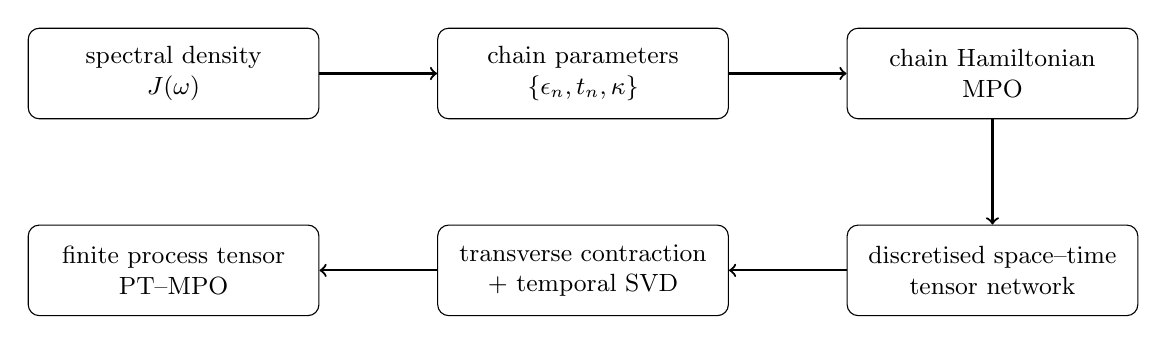
\begin{tikzpicture}[
        pipeline box/.style={
            draw,
            rounded corners,
            align=center,
            text width=3.2cm,
            minimum height=1.15cm,
            inner xsep=7pt,
            inner ysep=5pt,
            font=\small
        }
    ]
        \node[pipeline box] (spectrum) at (0,0)
            {spectral density\\\(J(\omega)\)};
        \node[pipeline box] (parameters) at (5.2,0)
            {chain parameters\\\(\{\epsilon_n,t_n,\kappa\}\)};
        \node[pipeline box] (chain) at (10.4,0)
            {chain Hamiltonian\\MPO};
        \node[pipeline box] (network) at (10.4,-2.5)
            {discretised space--time\\tensor network};
        \node[pipeline box] (contraction) at (5.2,-2.5)
            {transverse contraction\\+ temporal SVD};
        \node[pipeline box] (process) at (0,-2.5)
            {finite process tensor\\PT--MPO};

        \draw[->, thick] (spectrum.east) -- (parameters.west);
        \draw[->, thick] (parameters.east) -- (chain.west);
        \draw[->, thick] (chain.south) -- (network.north);
        \draw[->, thick] (network.west) -- (contraction.east);
        \draw[->, thick] (contraction.west) -- (process.east);
    \end{tikzpicture}
    \caption{Prospective chain-mapping route from a continuum spectral density to a finite temporal PT--MPO.}
    \label{fig:roadmap-chainmapping-pipeline}
\end{figure}
%
The existing Julia package \texttt{MPSDynamics.jl} already provides mature T-TEDOPA chain mappings and MPS dynamics for bosonic and fermionic environments~\cite{lacroix2024mpsdynamics}, and therefore provides a useful reference implementation and benchmark.
We would nevertheless favour a lightweight chain-mapping layer compatible with the current ITensors backend rather than make a second tensor-network framework a required dependency.

This direction is more ambitious than the ACE and PT-TEMPO extensions discussed above.
Its efficiency is controlled by the temporal entanglement generated during transverse contraction: the final influence functional may be compact even when intermediate tensors become substantially more entangled, and generic ergodic environments can require rapidly growing temporal bond dimensions~\cite{ye2021influence,cerezo2025spatiotemporal}.
Nevertheless, if this compression remains favourable, chain mapping would provide a powerful third route to finite PT--MPOs: ACE compresses explicitly separated bath modes, PT-TEMPO compresses analytically obtained Gaussian influence functions, while transverse chain contraction would construct the bath influence directly from an explicit many-body environment evolution.

\subsection{Quantum memory witness and Semi-Definite Programs}
\label{subsec:roadmap-quantum-memory}

\textcolor{red}{To be filled once Aaron's work is published.}
